\begin{scanpage}{0118}{101}
\noindent\begin{minipage}[t]{.48\linewidth}\vspace{0pt}\centering
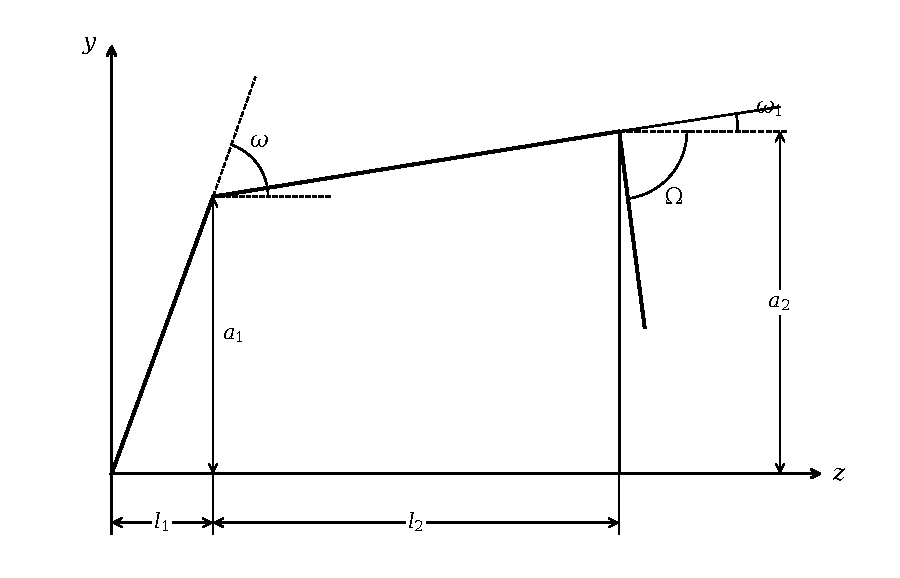
\includegraphics[width=.85\linewidth]{images/recreated/b-0118-fig34.pdf}

Figure 34. The generatrix of the surface of rotation.
\end{minipage}\hfill\begin{minipage}[t]{.48\linewidth}\vspace{0pt}\centering
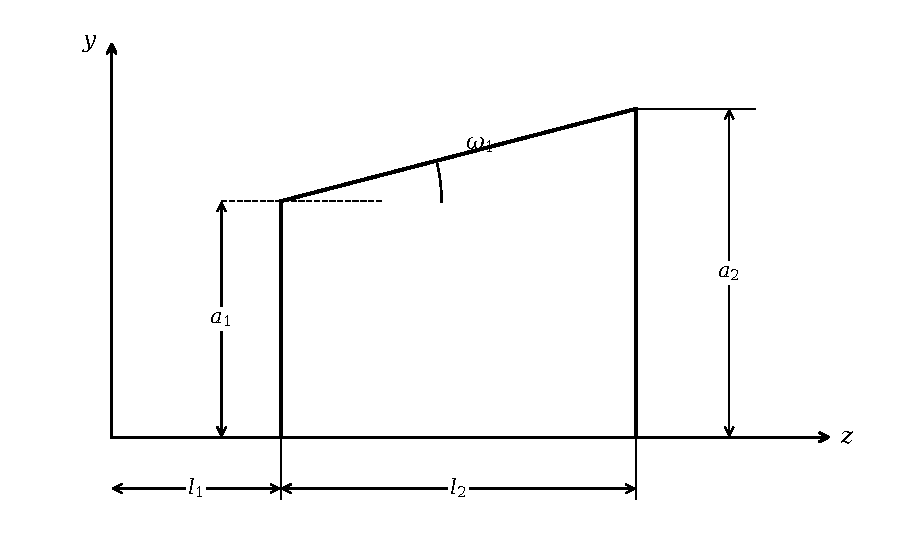
\includegraphics[width=.85\linewidth]{images/recreated/b-0118-fig35.pdf}

Figure 35. The generatrix of a truncated conical surface.
\end{minipage}\par\medskip

Summing this expressing with (17.02), where the quantities $l$ and $a$ must be replaced by $l_1$ and $a_1$, we find the field from the uniform part of the current flowing on the entire illuminated side of the body
\[\begin{aligned}E_x=-H_y=-\frac{a_1E_{0x}}2\biggl\{&\frac1{ka_1}\operatorname{tg}^2\omega\sin kl_1\,e^{ikl_1}-\operatorname{tg}\omega\,e^{2ikl_1}\\&+\left[\frac1{ka_1}\operatorname{tg}^2\omega_1\sin kl_2\,e^{ikl_2}+\left(1-\frac{a_2}{a_1}e^{2ikl_2}\right)\operatorname{tg}\omega_1\right]e^{2ikl_1}\biggr\}\frac{e^{ikR}}R.\end{aligned}\tag{17.17}\]
The field radiated by the nonuniform part of the current is determined in accordance with \S\ 16 by the equation
\[\begin{aligned}E_x=-H_y=-\frac{a_1E_{0x}}2\biggl[&\left(\frac{\frac2{n_1}\sin\frac\pi{n_1}}{\cos\frac\pi{n_1}-\cos\frac{2\omega}{n_1}}+\operatorname{tg}\omega-\operatorname{tg}\omega_1\right)e^{2ikl_1}\\&+\frac{a_2}{a_1}\left(\frac{\frac2{n_2}\sin\frac\pi{n_2}}{\cos\frac\pi{n_2}-\cos\frac{2\omega_1}{n_2}}+\operatorname{tg}\omega_1\right)e^{2ik(l_1+l_2)}\biggr]\frac{e^{ikR}}R,
\end{aligned}\tag{17.18}\]
where
\[n_1=1+\frac{\omega-\omega_1}\pi,\quad n_2=1+\frac{\omega_1+\Omega}\pi.\tag{17.19}\]
Now summing (17.17) and (17.18), we obtain a refined expression for the field scattered in the direction $\vartheta=\pi$
\[E_x=-H_y=-\frac{a_1E_{0x}}2\left(\frac1{ka_1}\operatorname{tg}^2\omega\sin kl_1\,e^{ikl_1}+\right.\tag{17.20}\]
\begin{center}(Equation continued on next page.)\end{center}
\end{scanpage}
